\section{Strato limite su placca piana}\label{c9}
La presente esercitazione si pone come obiettivo la caratterizzazione dello strato limite su placca piana mediante l'utilizzo dell'anemometria a filo caldo. In particolare, si vuole:
\begin{itemize}
    \item Misurare i profili di velocità per diverse ascisse $x$ con assegnata $U_\infty$;
    \item Caratterizzare la struttura dello strato limite:
    \begin{itemize}
        \item diagrammare i profili di velocità $u=u(x,y)$ e della deviazione standard delle fluttuazioni turbolente longitudinali $u_{rms}(x,y)$;
        \item valutare lo spessore geometrico $\delta(x)$, lo spessore di spostamento $\delta^*(x)$, lo spessore di quantità di moto $\theta(x)$ e il parametro di forma $H(x)$;
        \item verificare la condizione dello strato limite: laminare, transizionale o turbolento;
        \item diagrammare i profili di velocità media e fluttuante nella forma adimensionale: $u/U_\infty = f(y/\delta)$ e $u_{rms}/U_\infty = f(y/\delta)$.
    \end{itemize}
\end{itemize}

\subsection{Descrizione dell'esperimento}
A governare il campo di moto è il numero di Reynolds e in relazione al valore assunto localmente ($Re_{x}=U_\infty\cdot x/\nu$) lo strato limite può essere laminare oppure turbolento.
\begin{figure}[H]
    \centering
    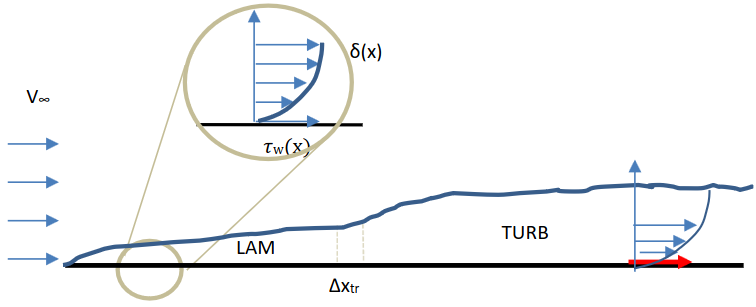
\includegraphics[width=.8\textwidth]{images/9/slimage.png}
    \caption{Rappresentazione dello strato limite}
\end{figure}

\noindent Se il numero di Reynolds locale supera il numero di Reynolds critico $Re_{cr}$ allora si ha strato limite turbolento, altrimenti si ha strato limite laminare. Dal numero di Reynolds critico si può quindi individuare la coordinata $x_{tr}$ di transizione:
\begin{equation*}
    Re_{cr}=\frac{U_\infty \cdot x_{tr}}{\nu}=5\cdot10^5
\end{equation*}
Per una placca piana posta ad incidenza nulla in un flusso senza turbolenza il numero di Reynolds critico vale $Re_{cr}\approx5\cdot10^5$. Se invece è presente turbolenza la transizione dello strato limite è anticipata, pertanto il numero di Reynolds critico risulta inferiore.\\\\
Per una data lunghezza $L$ della placca e conoscendo il valore della velocità della corrente a monte è possibile definire il numero di Reynolds globale della placca:
\begin{equation*}
    Re_L = \frac{U_\infty \cdot L}{\nu}
\end{equation*}
Nel caso di strato limite laminare la soluzione delle equazioni porta alla soluzione di Blasius, che definisce il profilo di velocità adimensionale sotto forma di tabella:
\begin{equation*}
    \eta(x,y) \approx \frac{y}{\delta(x)} = y\sqrt{\frac{U_\infty}{\nu x}} \qquad f^\prime = \frac{u}{V_\infty}
\end{equation*}
Per lo strato limite laminare sono valide le seguenti relazioni empiriche:
\begin{equation*}
    \delta(x) = \frac{5x}{\sqrt{Re_x}} \qquad \delta^*(x) = \frac{1.73x}{\sqrt{Re_x}} \qquad \theta(x) = \frac{0.664x}{\sqrt{Re_x}} \qquad H(x) = \frac{\delta^*}{\theta}
\end{equation*}
\begin{equation*}
    \tau_w(x) = 0.332 \sqrt{\frac{\rho \mu U_\infty^3}x} \qquad c_f(x) = \frac{0.664}{\sqrt{Re_x}} \qquad c_D = \frac{1.328}{\sqrt{Re_L}}
\end{equation*}
Nel caso di strato limite turbolento è presente una struttura multi-strato costituita principalmente da due regioni: inner layer ed outer layer.\\\\
L'inner layer, che copre una frazione pari al 10\%-20\% dello spessore dello strato limite $\delta$, a sua volta è costituito da tre substrati: il sottostrato viscoso, il buffer layer e la regione logaritmica.
\begin{figure}[H]
    \centering
    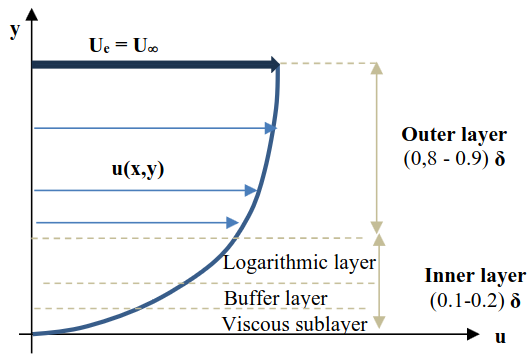
\includegraphics[width=.55\textwidth]{images/9/sltimage.png}
    \caption{Rappresentazione del profilo di velocità in uno strato limite turbolento}
\end{figure}




Lo strato limite turbolento è caratterizzato da una quantità di moto elevata e maggiore rispetto al laminare vicino a parete. Possiede quindi un gradiente di velocità elevato. Questi ultimi danno origine a effetti viscosi che si traducono quindi in sforzi viscosi a parete $\tau _w = \frac{du}{dY}|_{y = 0}$.\\
Per lo strato limite turbolento vengono definite due variabili caratteristiche
\begin{align*}
    u_{\tau} &= \sqrt{\frac{\tau_w}{\rho}} \quad \text{velocità d'attrito} \\
    \delta_v &= \frac{\nu}{u_\tau} \quad \text{lunghezza d'attrito}
\end{align*}

Con esse si possono adimensionalizzare $u(y)$ e $y$ e si 
\begin{align*}
    u^+ &= \sqrt{\frac{u}{u_\tau}} \quad  \\
    y^+ &= \frac{y}{\delta _v} \quad 
\end{align*}
Dato che si tratta di strato limite turbolento la velocità è di tipo media nel tempo. Con la lunghezza adimensionalizzata si possono distinguere gli strati che caratterizzano lo strato limite. Principalmente è composta dall'inner layer e dall'outer layer. Il primo ricopre circa il 20\% dello strato limite ed è ulteriormente suddviso in tre strati: viscous, buffer e log layer.

Per ognuna di queste regioni si definisce un'opportuna legge di distribuzione della velocità $u^+ = f(y^+)$:
\begin{itemize}
    \item Viscous sublayer: $0 \le y^+ \le \approx 5$\\
    Dominano gli effeti viscosi per gli elevati gradienti di velocità.
    \begin{equation*}
        u^+ = y^+
    \end{equation*}
    \item Buffer layer: $5 \le y^+ \le \approx 30$\\
    E' una zona di raccordo tra il sottostrato viscoso e la regione logaritmica
    \item Log layer: $30 \le y^+ \le \approx 1000$\\
    La velocità segue un preciso andamento 
    \begin{equation*}
        u^+ = \frac{1}{k}log(y^+) + B
    \end{equation*}
    con $k \approx 0.41$ e $B \approx 5.2$
    \item Outer layer: $y^+ > 1000$\\
    Il profilo inizia a seguire l'andamento del flusso esterno raccordandosi con esso
\end{itemize}

% \subsection{Catena di misura}
% Viene posta una placca piana della test section di una galleria del vento a circuito aperto. La placca tocca le pareti in modo da rendere il flusso più bidimensionale possibile. Si è certi che non avverranno fenomeni di bloccaggio in quanto la sezione frontale è decisamente minore rispetto alla sezione della test section.\\
% La sonda a filo caldo è posizionata su un movimentatore elettromeccanico con una sensibilità di 1 mm ogni 200 passi. Per ogni passo avviene quindi una traslazione di $5 \mu m$. Ogni esperimento viene effettuata a coordinata longitudinale fissata. Ricavato il segnale elettrico di tensione E attraverso la legge di taratura di King con le seguenti costanti di taratura.

% \begin{align*}
%     E^2 = A + BU^n \quad \text{Legge di King}\\
% \end{align*}

% \begin{align*}
% A = 2.0061\\
% B = 0.6671\\
% n = 0.518 
% \end{align*}

% E' quindi possibile ricavare la velocità di raffreddamento $u(x,y)$. Il segnale prima di approdare nel PC verrà eleborato attraverso il sistema di elaborazione dati.


% \subsection{Procedura sperimentale}
% L'esperimento consiste di posizionare la sonda in una specifica posizione che cambia da squadra a squadra. Dopodichè si imposta una certa velocità per osservare lo strato limite laminare per poi cambiare velocità in modo da analizzare anche quello turbolento.\\
% La sonda viene posta il più vicino possibile alla placca facendo attenzione che non la tocchi. Infatti la sonda viene posta a qualche decimo di millimetro in modo da evitare che le vibrazioni a cui sarà sottoposta la sonda durante l'esperimento non la portano a rompersi toccando la placca.\\
% In primo luogo viene rilevato il valore di offset a wind off, cioò a galleria spenta. Attivata quindi la galleria e dopo aver atteso il transitorio per ottenere una velocità costante in galleria si procede con le misurazioni attraverso la movimentazione nella coordinata trasversale della sonda. \\
% Si campiona con una frequenza $f_s = 200 Hz$ per 30 secondi ad altezza. In questo modo si ottengono 6000 misurazioni. 

% \subsection{Analisi dati}
% Di seguito vengono presentati i dati grezzi della squadra 3

% Per ogni stazione di acquisizione si calcola il valore medio e di conseguenza anche la deviazione standard

% \begin{equation*}
%     \Bar{U} = \frac{1}{N_s}\sum_{j=1}^{N_s} U_j
% \end{equation*}

% \begin{equation*}
%     u_{rms} = \frac{1}{N_s}\sum_{j=1}^{N_s}\sqrt{(U - \Bar{U})^2}
% \end{equation*}

% Lo spessore dello strato limite coincide con la velocità pari al 99\% di quella del flusso esterno. In particolare si è imposta una velocità esterna nel primo esperimento pari a 3.47884 m/s e nel secondo esperimento pari a 11.1159 m/s che corrispondono al caso di strato limite laminare e turbolento. In particolare calcolano i Reynolds locali $Re_x = \frac{U_\infty x}{\nu}$ si nota che il primo esperimento ha dato origine ad una condizione di strato limite turbolento mentre il secondo esperimento è sicuramente laminare dato che il Reynolds risiede sotto il valore di 500000. \\
% Di seguito vengono quindi esposti i due casi.
% \subsection{Strato limite laminare}
% \subsubsection{Profilo di velocità media e fluttuazioni di velocità}
% Vengono visualizzati i profili per la velocità media


% e per le fluttuazioni di velocità

% \subsubsection{Grandezze notevoli dello strato limite}
% Dal grafico di velocità media si può quindi ricavare lo spessore geometrico dello strato limite laminare $\delta = 2.2 \ mm$.\\
% Per quanto riguarda lo spessore di spostamento:

% \begin{equation*}
%     \delta^* = \int_{\infty}^{0} \left(1 - \frac{u}{U_e}\right) \, dy = 3.449
%  \ mm
% \end{equation*}

% Lo spessore di quantità di moto

% \begin{equation*}
%     \theta = \int_{\infty}^{0} \frac{u}{U_e} \cdot\left(1 - \frac{u}{U_e}\right) \, dy = 1.918 \ mm
% \end{equation*}

% E infine il parametro di forma

% \begin{equation*}
%     H = \frac{\delta^*}{\theta} = 1.798 \ mm
% \end{equation*}

% \subsubsection{Profili di velocità media e fluttuazioni adimensionali}

% Vengono presentate le velocità medie e le fluttuazioni adimensionalizzate rispettivamente come 

% \begin{equation*}
%     \frac{u}{U_{\infty}} = f \left( \frac{y}{\delta} \right)
% \end{equation*}

% \begin{equation*}
%     \frac{u_{\text{rms}}}{U_{\infty}} = f \left( \frac{y}{\delta} \right)
% \end{equation*}

% \subsubsection{Confronto con la teoria di Blausius}
% Viene costruita una variabile adimensionale $\eta = \frac{y}{\delta}$ con $\delta$ spessore geometrico.\\
% E' possibile quindi esprimere le equazioni del moto come

% \begin{equation*}
%     ff^{''} + 2 f^{'''} = 0
% \end{equation*}

% con $f = f(\eta)$ e $f^{'} = \frac{u}{U_\infty}$. Si ottiene una soluzione tabulata che viene riportata in appendice. Si denota comunque che fino a un certo numero di Reynolds, cioè fino a quando lo strato limite è da considerarsi laminare, si ha una soluzione unica per i profili di velocità. E' come se il flusso fosse self-similare.\\
% Di seguito viene presentato il confronto tra i dati sperimentali e la soluzione di Blausius

% \subsection{Strato limite turbolento}
% \subsubsection{Profilo di velocità media e fluttuazioni di velocità}
% Si presentano i profili dei sperimentali relativi alle velocità medie e alle fluttuazioni di velocità

% \subsubsection{Grandezze notevoli dello strato limite}
% Dal grafico di velocità media anche per il caso turbolento si può ricavare lo spessore geometrico dello strato limite laminare $\delta = 5.05 \ mm$.\\
% Per quanto riguarda lo spessore di spostamento:

% \begin{equation*}
%     \delta^* = \int_{\infty}^{0} \left(1 - \frac{u}{U_e}\right) \, dy = 0.204 \ mm 
% \end{equation*}

% Lo spessore di quantità di moto

% \begin{equation*}
%     \theta = \int_{\infty}^{0} \frac{u}{U_e} \cdot\left(1 - \frac{u}{U_e}\right) \, dy = 1.7 \ mm
% \end{equation*}

% E infine il parametro di forma

% \begin{equation*}
%     H = \frac{\delta^*}{\theta} = 1.201 \ mm
% \end{equation*}

% \subsubsection{Profili di velocità media e fluttuazioni adimensionali}

%  Le velocità medie e le fluttuazioni adimensionalizzate nel caso turbolento con la medesima adimensionalizzazione del caso laminare si presentano come:

% \subsubsection{Diagramma con variabili interne dello strato limite}
% Si sfrutta il Metodo di Clauser per tracciare i profili di velocità media e delle fluttuazioni adimensionalizzati con le variabili interne dello strato limite.

% \begin{equation*}
%     u^+ = \frac{\Bar{U}}{u_\tau} = f(y^+)
% \end{equation*}

% \begin{equation*}
%     \frac{u_{rms}}{u_\tau} = f(y^+)
% \end{equation*}

% Le variabili interne dello strato limite turbolento si definiscono come:

% \begin{equation*}
%     y^+ = \frac{y}{l_\tau}
% \end{equation*}

% \begin{equation*}
%         l_\tau = \frac{\nu}{u_\tau} \\
% \end{equation*}

% \begin{equation*}
%     u_\tau = \frac{\tau _w}{\rho} = U_e \sqrt{\frac{Cf}{2}}
% \end{equation*}
% Attraverso il metodo di Clauser è possibile determinare il valore del coefficiente di sforzo d'attrito a parete $C_f = \frac{\tau _w}{\frac{1}{2}\rho U^2_e}$.\\
% In questo metodo viene sfruttato il log layer per conoscere lo strato interno dello strato limite turbolento e quindi per determinare in modo sommario lo sforzo d'attrito a parete. Infatti nel log layer c'è la possibilità di avere più misurazioni che inoltre sono più accurate.\\
% Sfruttando quindi la relazione della velocità nel sottostrato logaritmico 

% \begin{equation*}
%     u^+ = \frac{1}{k}logy^+ + C
% \end{equation*}

% con k = 0.41 (costante di VonKarman) e C = 5.1 (costante di Coles). Utilizzando le relazione di $u^+$ e $y^+$ si ottiene la seguente formulazione:

% \begin{equation*}
%     \frac{u}{U_e} = \sqrt{\frac{Cf}{2}}\left[\frac{1}{k}\left(log\frac{yU_e}{\nu} + log\sqrt{\frac{C_f}{2}}\right) + C\right]
% \end{equation*}

% Viene quindi costruita la mappa di Clauser assumendo differenti valori di $C_f$. Sovrapponendo il profilo di velocità sperimentale si osserva quale $C_f$ si avvicina maggiormente ai dati sperimentali.

% Si ricava quindi il $C_f = 0.0045$ con il quale si rappresenta l'andamento della velocità e delle fluttuazioni all'interno dello strato limite

% \begin{equation*}
%     u^+ = \frac{U}{u_\tau}
% \end{equation*}

% \begin{equation*}
%     y^+ = \frac{y}{l_\tau}
% \end{equation*}

% Si ottiene quindi il seguente diagramma per la velocità adimensionale rispetto alla coordinata interna


% Per quanto riguarda le fluttuazioni invece:

% \subsection{Confronto strato limite laminare e turbolento}

% In primo luogo si evidenzia il confronto tra i valori notevoli dello strato limite laminare e turbolento:


% Vengono dati anche i grafici di confronto tra gli andamenti dello strato limite laminare e turbolento per la velocità media, le fluttuazioni turbolente e i valori adimensionali.